\graphicspath{{Figures/RAA/}}


\section{\label{RAA}Nuclear modification factor}

The \ups nuclear modification factor (\Raa) is computed such as:
\begin{align*}
%\label{RaaShort}R^{i}_{\rm{AA}}&=\frac{{\rm d}^{2}Y^{{\rm PbPb},\;i}_{\jpsi}/{\rm d}\pt{\rm d}y}{\langle T^{i}_{\rm AA}\rangle\;{\rm d}^{2}\sigma^{\rm{pp}}_{\jpsi}/{\rm d}\pt{\rm d}y} \\
R^{i}_{\rm{AA}}=\frac{{\rm d}^{2}N^{{\rm measured},\;i}_{\ups}/{\rm d}\pt{\rm d}y}{\langle T^{i}_{\rm AA}\rangle\;BR_{\ups\to\mu^{+}\mu^{-}}\;A\epsilon^{i}\;N^{{\rm MB},\;i}_{evt}\;{\rm d}^{2}\sigma^{\rm{pp}}_{\ups}/{\rm d}\pt{\rm d}y}.
\end{align*}
where:
\begin{itemize}
\item $N^{{\rm measured},\;i}$ is the number of \ups measured in the centrality bin $i$ (cf \ref{NUps}),
\item $\langle T^{i}_{\rm AA}\rangle$ is the nuclear overlap function (\href{https://twiki.cern.ch/twiki/bin/view/ALICE/CentralityCodeSnippets#Anchor_Point}{values}),
\item $BR_{\ups\to\mu^{+}\mu^{-}}$ is the branching ratio of \ups decaying in two muons (2.48\%),
\item $A\epsilon^{i}$ is the acceptance times efficiency correction of the muon spectrometer (cf \ref{AccEffValues}),
\item $N^{{\rm MB},\;i}_{evt}$  represent the equivalent number of Minimum Bias events with respect to the number of dimuon triggered events (CMUL) by taking into account its dead time (cf \ref{Fnorm}),
\item $\sigma^{\rm{pp}}_{\ups}$ is the \ups pp cross section at \sqrtSE[5.02][TeV].
\end{itemize}


\paragraph{\label{Fnorm}$\boldsymbol{N^{{\rm MB}}}$}
The equivalent number of MB events is obtained run by run via the determination of the normalization factor ($F_{\rm norm}$) describes in the charmonium analysis note of the same data taking period and available \href{https://aliceinfo.cern.ch/Notes/node/486}{here}.
The mean value of the normalization factor over the full period is equal to $11.84 \pm 0.01(stat.)$ for the centrality class 0-90\%.
Finally a total number of $1.5\ldotp10^9$ MB events within 0-90\% centrality class is analyzed.


\paragraph{$\boldsymbol{\sigma^{\rm{pp}}_{\ups}}$}
The \ups pp reference has been estimated by extrapolation from different models and from LHCb and ALICE measurements at lower and higher energies.
A common public note has been published (\href{https://cds.cern.ch/record/1748460?ln=fr}{CDS}).
The values reported in table \ref{sigmapp} have been computed for the rapidity region cover by the muon spectrometer ($-4<y<-2.5$) and three rapidity points which correspond to 2.75, 3.25 and 3.75.

\begin{table}[htb]
  \centering
  \begin{tabular} { c | c }
    \hline
    \y & $\sigma^{\rm{pp}}_{\ups}$ (nb)  \\\hline
    $[2.5-4]$ & $1.14 \pm 0.10 \;(8.8\%)$ \\
    $[2.5-3]$ & $ 0.484 \pm 0.038 \;(7.9\%) $ \\
    $[3-3.5]$ & $ 0.376 \pm 0.045 \;(12.0\%) $ \\
    $[3.5-4]$ & $ 0.257 \pm 0.029 \;(11.3\%) $ \\\hline
  \end{tabular}
  \caption{\label{sigmapp}\ups pp cross section at \sqrtSE[5.02][TeV] computed by extrapolation.} 
\end{table}


\paragraph{$\boldsymbol{A\epsilon}$}
The spectrometer correction of acceptance times efficiency is computed in the embedding MC (production LHC16e2 \& plus), thus we are able to reproduce the realistic occupancy of the muon tracking chambers as a function of the collision centrality.
A total of  1 937 708 \ups has been embedded in CINT7-B-NOPF-MUFAST events.
Two scaling have to be achieved in order to get the proper $A\epsilon$ correction:
\begin{itemize}
\item as a function of the number of CMUL events analyzed per run to account for the time evolution of the apparatus and the relative statistic available,
\item as a function of the collision centrality by using the mean number of binary collisions because the centrality distribution of CINT7 events is flat unlike the CMUL7 events.
\end{itemize}
The $A\epsilon$ results are shown as a function of the run number, the collision centrality, the \ups $y$ and \pt on figure \ref{AccEffplots}.
We can observe a good stability of the muon spectrometer capabilities in time.
A drop of around 8\% of the $A\epsilon$ is observe going from peripheral to central collisions as expected and already seen in previous data.
Finally an integrated \ups correction of $26.35\pm0.03(stat.)$\% has been found.
The centrality and rapidity dependence results are reported in the table \ref{AccEffValues}.

\begin{table}[htb]
  \centering
  \begin{tabular} { c | c | c | c}
    \hline
    centrality & $A\epsilon \pm (stat.)$ (\%) &  \y & $A\epsilon \pm (stat.)$ (\%)\\\hline
    0-10\% &  $ 25.61 \pm 0.09 $   &  $[2.5-3]$ & $19.56 \pm 0.04$ \\
    10-30\% & $ 26.68 \pm 0.07 $  & $[3-3.5]$ & $ 39.73 \pm  0.06 $ \\
    30-50\% & $ 27.29 \pm 0.07 $ & $[3.5-4]$ & $ 19.95 \pm  0.029 $ \\
    50-90\% & $ 27.63 \pm 0.05 $  &  \\
    0-20\% & $ 25.97 \pm 0.07 $   &  & \\
    20-90\% & $ 27.15 \pm 0.04 $   &  & \\\hline
  \end{tabular}
  \caption{\label{AccEffValues}\ups $A\epsilon$ correction values for the centrality and rapidity intervals under study and obtained from embedding MC. The statistical uncertainties quoted here and related to the deep of the MC sample are negligible.} 
\end{table}

\begin{figure}[!t]
\begin{center}
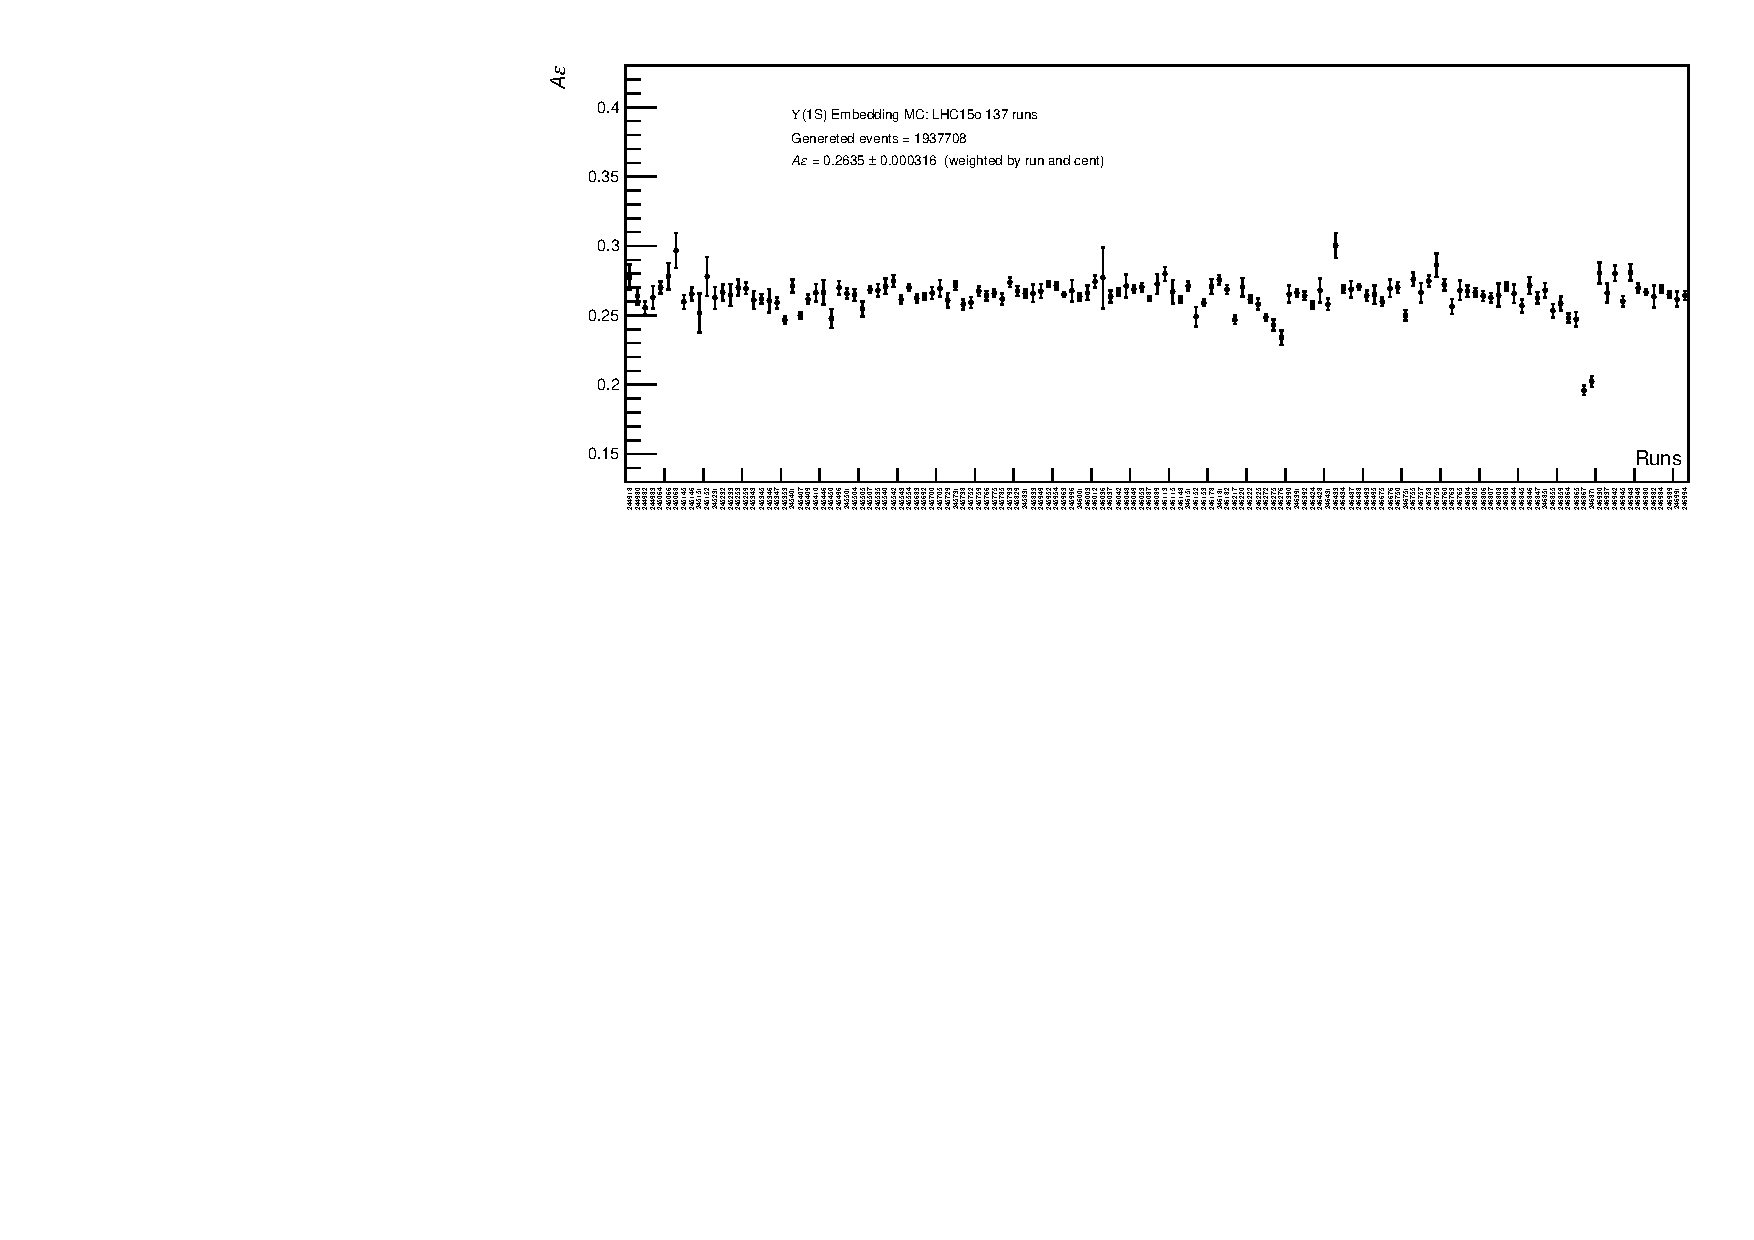
\includegraphics[width=13cm]{/AxE/Antoine/AccEffvsRun_LHC15o_137runs_MUL_pt_0_y_0.pdf}
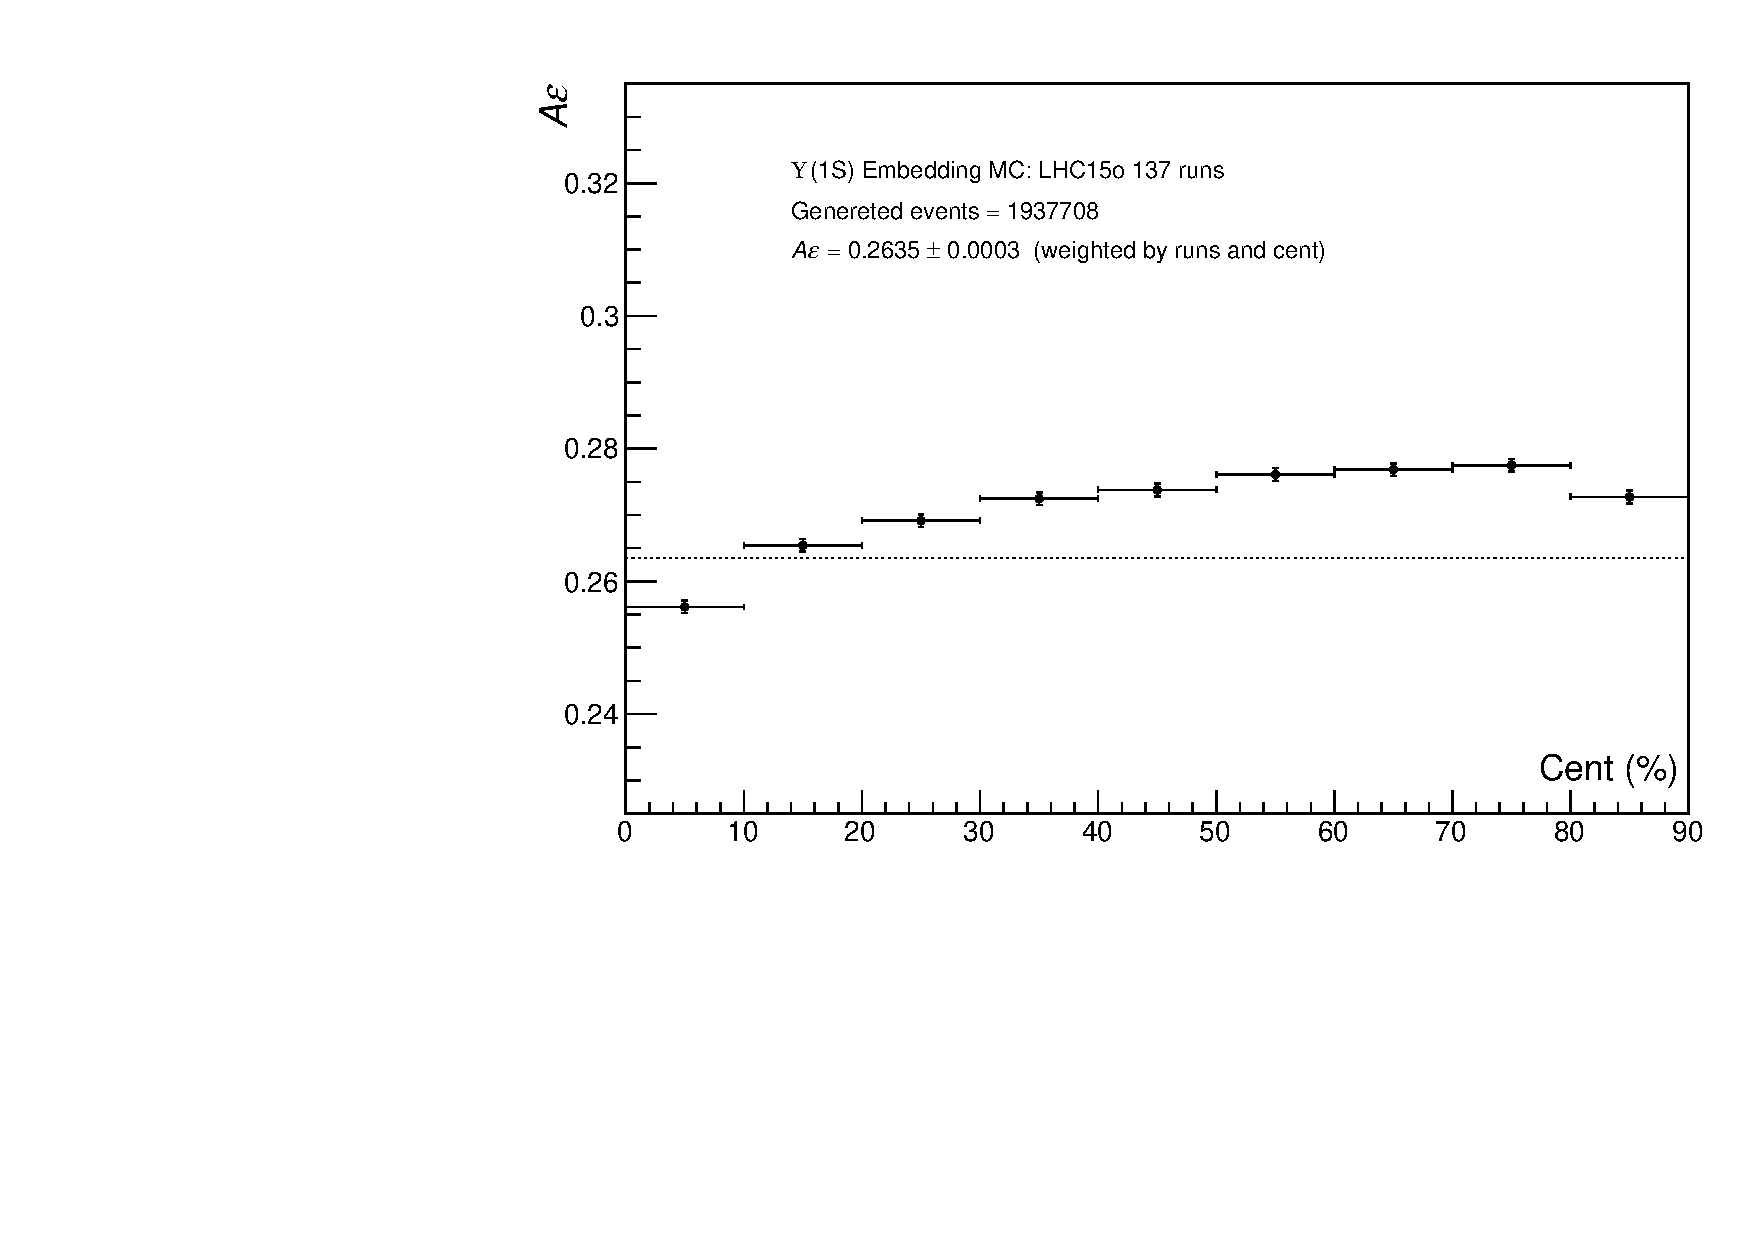
\includegraphics[width=6cm]{/AxE/Antoine/AccEffvsCent_LHC15o_137runs_MUL_pt_0_y_0.pdf}\\
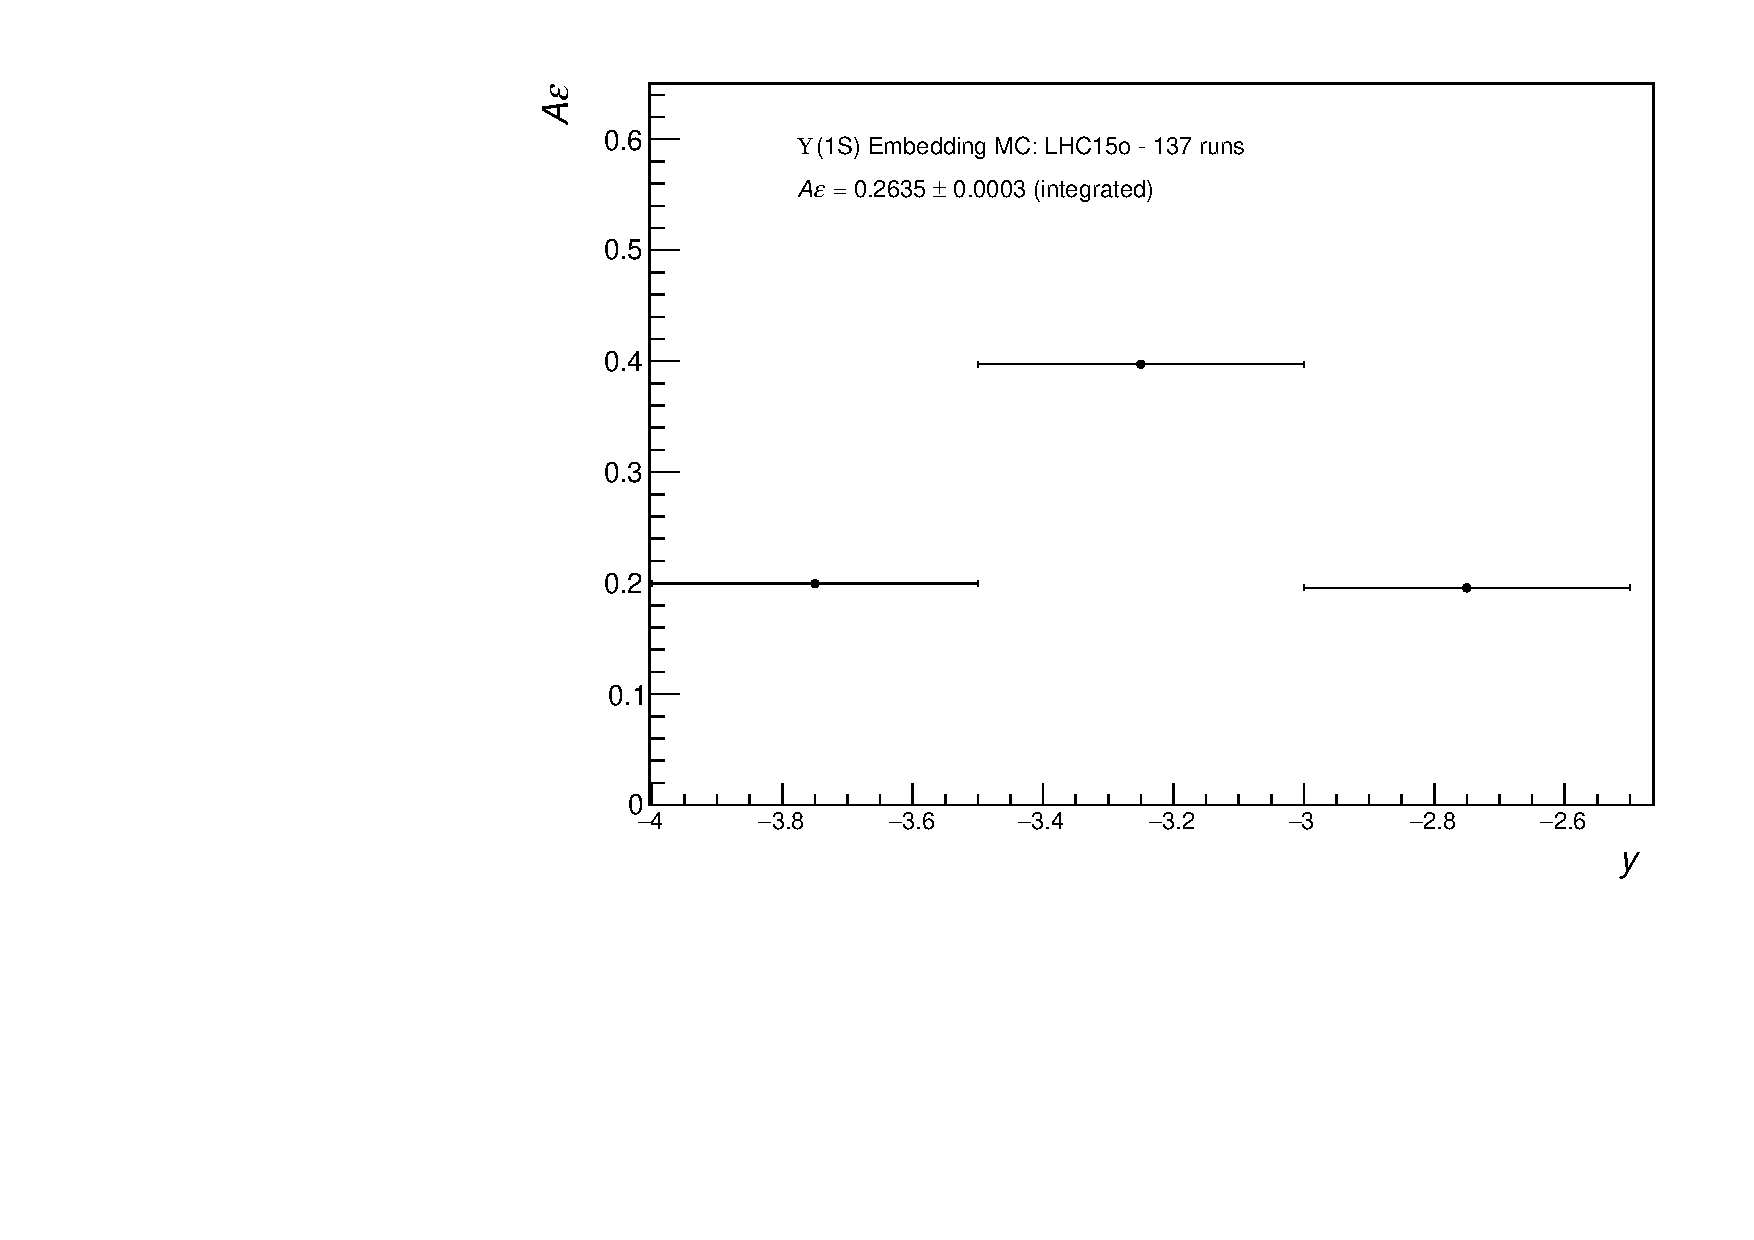
\includegraphics[width=6cm]{/AxE/Antoine/AccEffvsY_LHC15o_137runs_weighted.pdf}
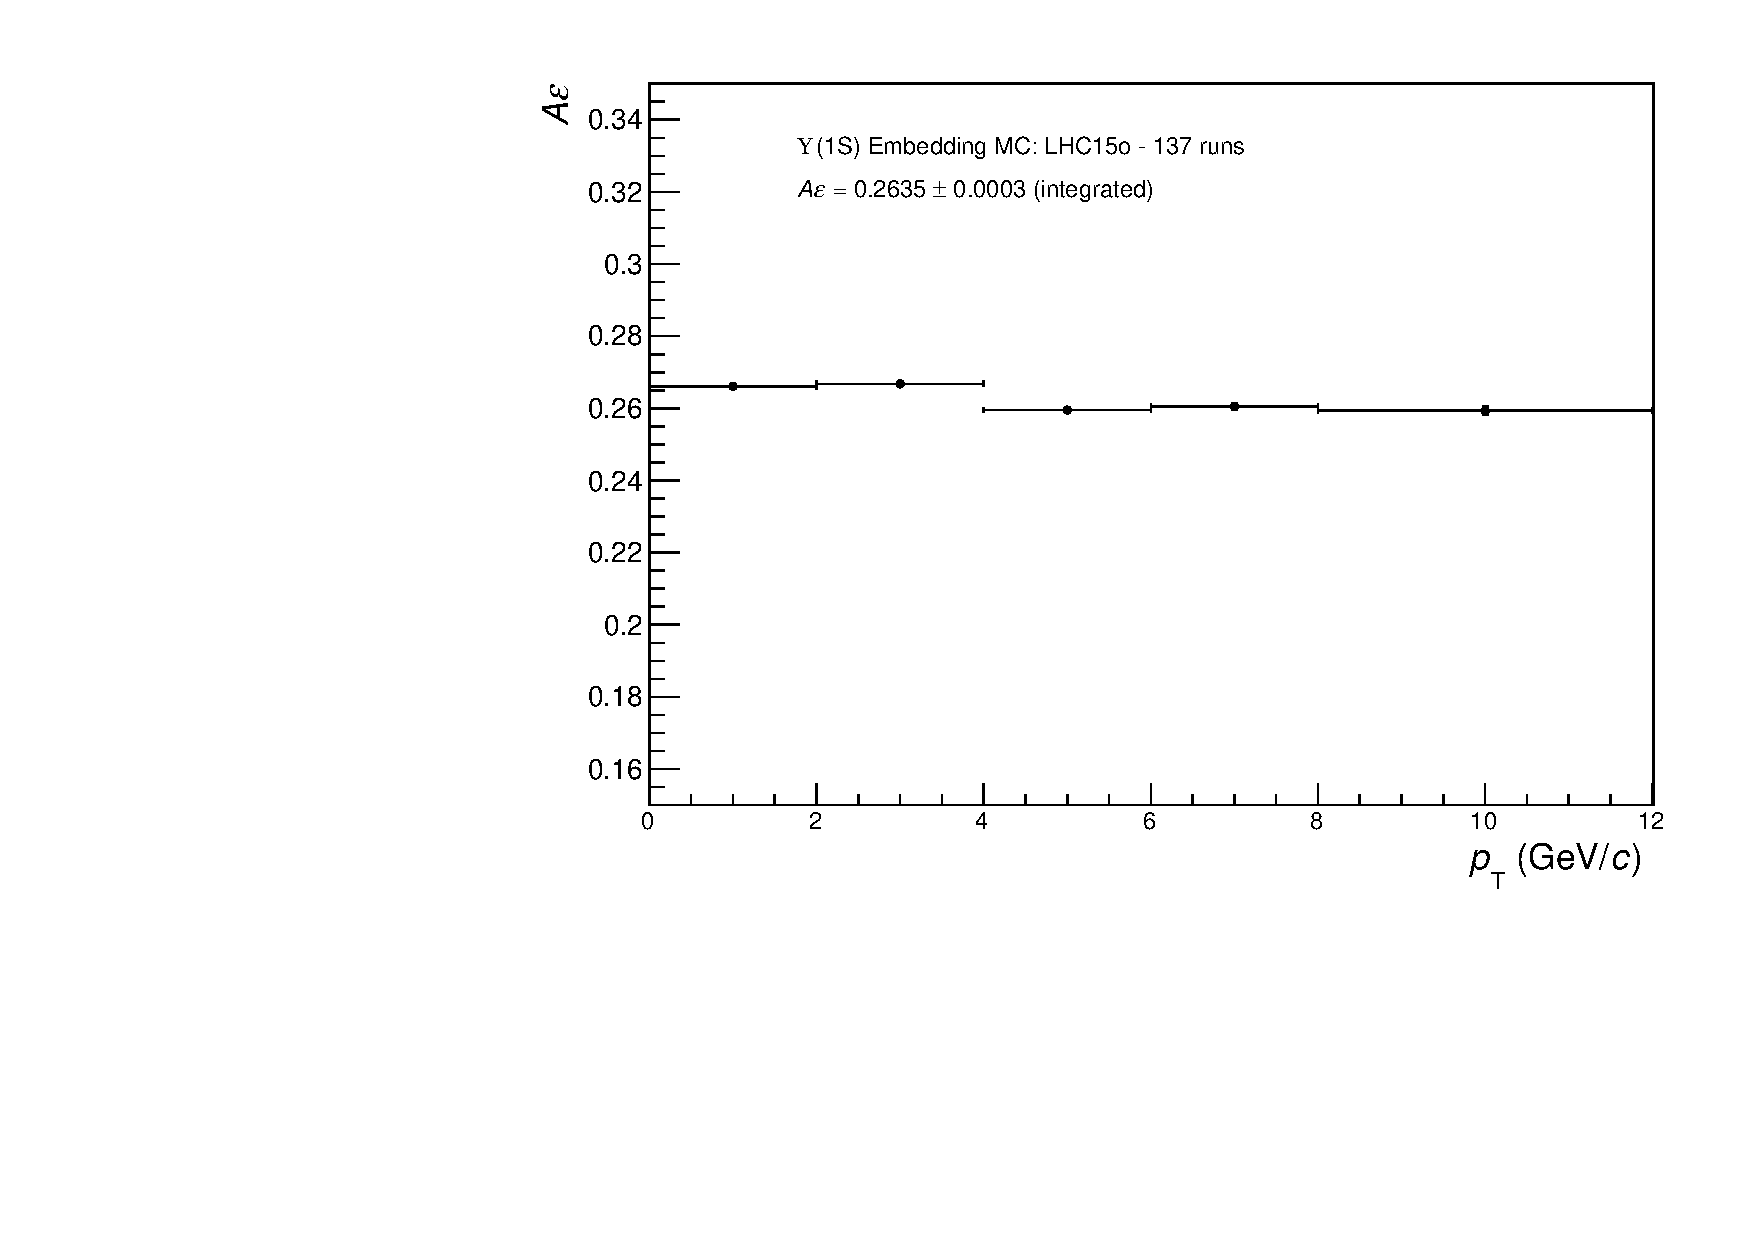
\includegraphics[width=6cm]{/AxE/Antoine/AccEffvsPt_LHC15o_137runs_weighted.pdf}
\end{center}
\caption{\label{AccEffplots}$A\epsilon$ correction extracted from embedding MC as a function of the run number (top), the collision centrality (center), the \ups rapidity (bottom left) and the \ups transverse momentum (bottom right).}
\end{figure}
